%%%------------------------------------------------------------------------------------------------------------
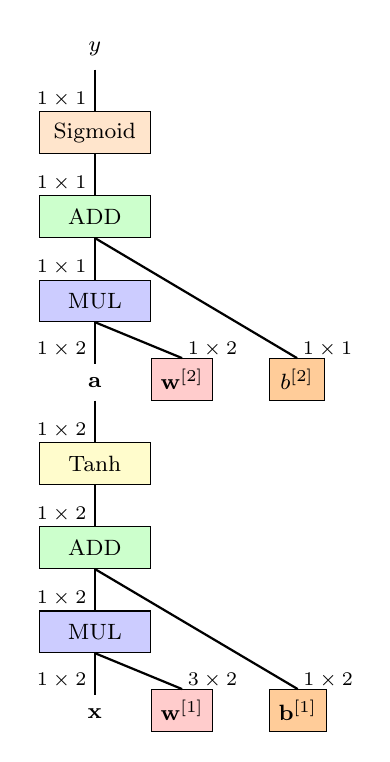
\begin{tikzpicture}

\node [anchor=west,minimum width=1.5em,minimum height=1.5em] (part1) at (0,0) {\footnotesize{$y$}};
\node [anchor=north,minimum width=1.5em,minimum height=1.5em] (part1-2) at ([xshift=-1.2em,yshift=-0.3em]part1.south) {\scriptsize {$1\times1$}};
\node [anchor=north,draw,minimum width=4.0em,minimum height=1.5em,fill=orange!20] (part2) at ([yshift=-1.5em]part1.south) {\footnotesize {$\rm{Sigmoid}$}};
\draw [-,thick](part1.south)--(part2.north);

\node [anchor=north,minimum width=1.5em,minimum height=1.5em] (part2-2) at ([xshift=-1.2em,yshift=-0.3em]part2.south) {\scriptsize {$1\times1$}};
\node [anchor=north,draw,minimum width=4.0em,minimum height=1.5em,fill=green!20] (part3) at ([yshift=-1.5em]part2.south) {\footnotesize {$\rm{ADD}$}};
\draw [-,thick](part2.south)--(part3.north);

\node [anchor=north,minimum width=1.5em,minimum height=1.5em] (part3-2) at ([xshift=-1.2em,yshift=-0.3em]part3.south) {\scriptsize {$1\times1$}};
\node [anchor=north,draw,minimum width=4.0em,minimum height=1.5em,fill=blue!20] (part4) at ([yshift=-1.5em]part3.south) {\footnotesize {$\rm{MUL}$}};
\draw [-,thick](part3.south)--(part4.north);

\node [anchor=north,minimum width=1.5em,minimum height=1.5em] (part4-2) at ([xshift=-1.2em,yshift=-0.2em]part4.south) {\scriptsize {$1\times 2$}};
\node [anchor=north,minimum width=4.0em,minimum height=1.5em] (part5) at ([yshift=-1.4em]part4.south) {\footnotesize {$\mathbf a$}};
\draw [-,thick](part4.south)--([yshift=-0.1em]part5.north);
%%%%%%%%%%%%%%%%%%%%%%%%%%%%
\node [anchor=west,minimum width=2.0em,minimum height=1.5em,draw,fill=red!20] (part5-3) at ([xshift=0.0em,yshift=0.1em]part5.east) {\footnotesize {$\mathbf w^{[2]}$}};
\node [anchor=west,minimum width=2.0em,minimum height=1.5em,draw,fill=orange!40] (part5-4) at ([xshift=2.0em,yshift=0.0em]part5-3.east) {\footnotesize {$ b^{[2]}$}};
\draw[-,thick](part4.south)--(part5-3.north);
\draw[-,thick](part3.south)--(part5-4.north);
\node [anchor=south,minimum width=1.5em,minimum height=1.5em] (part5-3-1) at ([xshift=1.1em,yshift=-0.45em]part5-3.north) {\scriptsize {$1\times 2$}};
\node [anchor=south,minimum width=1.5em,minimum height=1.5em] (part5-4-1) at ([xshift=1.1em,yshift=-0.45em]part5-4.north) {\scriptsize {$1\times1$}};
%%%%%%%%%%%%%%%%%%%%%%%%%%
\node [anchor=north,minimum width=1.5em,minimum height=1.5em] (part5-2) at ([xshift=-1.2em,yshift=-0.2em]part5.south) {\scriptsize {$1\times 2$}};
\node [anchor=north,draw,minimum width=4.0em,minimum height=1.5em,fill=yellow!20] (part6) at ([yshift=-1.4em]part5.south) {\footnotesize {$\rm{Tanh}$}};
\draw [-,thick]([yshift=0.1em]part5.south)--(part6.north);

\node [anchor=north,minimum width=1.5em,minimum height=1.5em] (part6-2) at ([xshift=-1.2em,yshift=-0.3em]part6.south) {\scriptsize {$1\times 2$}};
\node [anchor=north,draw,minimum width=4.0em,minimum height=1.5em,fill=green!20] (part7) at ([yshift=-1.5em]part6.south) {\footnotesize {$\rm{ADD}$}};
\draw [-,thick](part6.south)--(part7.north);

\node [anchor=north,minimum width=1.5em,minimum height=1.5em] (part7-2) at ([xshift=-1.2em,yshift=-0.3em]part7.south) {\scriptsize {$1\times 2$}};
\node [anchor=north,draw,minimum width=4.0em,minimum height=1.5em,fill=blue!20] (part8) at ([yshift=-1.5em]part7.south) {\footnotesize {$\rm{MUL}$}};
\draw [-,thick](part7.south)--(part8.north);

\node [anchor=north,minimum width=1.5em,minimum height=1.5em] (part8-2) at ([xshift=-1.2em,yshift=-0.2em]part8.south) {\scriptsize{$1\times 2$}};
\node [anchor=north,minimum width=4.0em,minimum height=1.5em] (part9) at ([yshift=-1.4em]part8.south) {\footnotesize {$\mathbf x$}};
\draw [-,thick](part8.south)--([yshift=-0.1em]part9.north);
%%%%%%%%%%%%%%%%%%%%%%%%%%%%
\node [anchor=west,minimum width=2.0em,minimum height=1.5em,draw,fill=red!20] (part9-3) at ([xshift=0.0em,yshift=0.1em]part9.east) {\footnotesize {$\mathbf w^{[1]}$}};
\node [anchor=west,minimum width=2.0em,minimum height=1.5em,draw,fill=orange!40] (part9-4) at ([xshift=2.0em,yshift=0.0em]part9-3.east) {\footnotesize {$\mathbf b^{[1]}$}};
\draw[-,thick](part8.south)--(part9-3.north);
\draw[-,thick](part7.south)--(part9-4.north);
\node [anchor=south,minimum width=1.5em,minimum height=1.5em] (part9-3-1) at ([xshift=1.1em,yshift=-0.45em]part9-3.north) {\scriptsize {$3\times 2$}};
\node [anchor=south,minimum width=1.5em,minimum height=1.5em] (part9-4-1) at ([xshift=1.1em,yshift=-0.45em]part9-4.north) {\scriptsize {$1\times 2$}};
%%%%%%%%%%%%%%%%%%%%%%%%%%

\end{tikzpicture}
%%------------------------------------------------------------------------------------------------------------




